% Options for packages loaded elsewhere
\PassOptionsToPackage{unicode}{hyperref}
\PassOptionsToPackage{hyphens}{url}
%
\documentclass[
]{article}
\usepackage{amsmath,amssymb}
\usepackage{lmodern}
\usepackage{iftex}
\ifPDFTeX
  \usepackage[T1]{fontenc}
  \usepackage[utf8]{inputenc}
  \usepackage{textcomp} % provide euro and other symbols
\else % if luatex or xetex
  \usepackage{unicode-math}
  \defaultfontfeatures{Scale=MatchLowercase}
  \defaultfontfeatures[\rmfamily]{Ligatures=TeX,Scale=1}
\fi
% Use upquote if available, for straight quotes in verbatim environments
\IfFileExists{upquote.sty}{\usepackage{upquote}}{}
\IfFileExists{microtype.sty}{% use microtype if available
  \usepackage[]{microtype}
  \UseMicrotypeSet[protrusion]{basicmath} % disable protrusion for tt fonts
}{}
\makeatletter
\@ifundefined{KOMAClassName}{% if non-KOMA class
  \IfFileExists{parskip.sty}{%
    \usepackage{parskip}
  }{% else
    \setlength{\parindent}{0pt}
    \setlength{\parskip}{6pt plus 2pt minus 1pt}}
}{% if KOMA class
  \KOMAoptions{parskip=half}}
\makeatother
\usepackage{xcolor}
\usepackage[margin=1in]{geometry}
\usepackage{color}
\usepackage{fancyvrb}
\newcommand{\VerbBar}{|}
\newcommand{\VERB}{\Verb[commandchars=\\\{\}]}
\DefineVerbatimEnvironment{Highlighting}{Verbatim}{commandchars=\\\{\}}
% Add ',fontsize=\small' for more characters per line
\usepackage{framed}
\definecolor{shadecolor}{RGB}{248,248,248}
\newenvironment{Shaded}{\begin{snugshade}}{\end{snugshade}}
\newcommand{\AlertTok}[1]{\textcolor[rgb]{0.94,0.16,0.16}{#1}}
\newcommand{\AnnotationTok}[1]{\textcolor[rgb]{0.56,0.35,0.01}{\textbf{\textit{#1}}}}
\newcommand{\AttributeTok}[1]{\textcolor[rgb]{0.77,0.63,0.00}{#1}}
\newcommand{\BaseNTok}[1]{\textcolor[rgb]{0.00,0.00,0.81}{#1}}
\newcommand{\BuiltInTok}[1]{#1}
\newcommand{\CharTok}[1]{\textcolor[rgb]{0.31,0.60,0.02}{#1}}
\newcommand{\CommentTok}[1]{\textcolor[rgb]{0.56,0.35,0.01}{\textit{#1}}}
\newcommand{\CommentVarTok}[1]{\textcolor[rgb]{0.56,0.35,0.01}{\textbf{\textit{#1}}}}
\newcommand{\ConstantTok}[1]{\textcolor[rgb]{0.00,0.00,0.00}{#1}}
\newcommand{\ControlFlowTok}[1]{\textcolor[rgb]{0.13,0.29,0.53}{\textbf{#1}}}
\newcommand{\DataTypeTok}[1]{\textcolor[rgb]{0.13,0.29,0.53}{#1}}
\newcommand{\DecValTok}[1]{\textcolor[rgb]{0.00,0.00,0.81}{#1}}
\newcommand{\DocumentationTok}[1]{\textcolor[rgb]{0.56,0.35,0.01}{\textbf{\textit{#1}}}}
\newcommand{\ErrorTok}[1]{\textcolor[rgb]{0.64,0.00,0.00}{\textbf{#1}}}
\newcommand{\ExtensionTok}[1]{#1}
\newcommand{\FloatTok}[1]{\textcolor[rgb]{0.00,0.00,0.81}{#1}}
\newcommand{\FunctionTok}[1]{\textcolor[rgb]{0.00,0.00,0.00}{#1}}
\newcommand{\ImportTok}[1]{#1}
\newcommand{\InformationTok}[1]{\textcolor[rgb]{0.56,0.35,0.01}{\textbf{\textit{#1}}}}
\newcommand{\KeywordTok}[1]{\textcolor[rgb]{0.13,0.29,0.53}{\textbf{#1}}}
\newcommand{\NormalTok}[1]{#1}
\newcommand{\OperatorTok}[1]{\textcolor[rgb]{0.81,0.36,0.00}{\textbf{#1}}}
\newcommand{\OtherTok}[1]{\textcolor[rgb]{0.56,0.35,0.01}{#1}}
\newcommand{\PreprocessorTok}[1]{\textcolor[rgb]{0.56,0.35,0.01}{\textit{#1}}}
\newcommand{\RegionMarkerTok}[1]{#1}
\newcommand{\SpecialCharTok}[1]{\textcolor[rgb]{0.00,0.00,0.00}{#1}}
\newcommand{\SpecialStringTok}[1]{\textcolor[rgb]{0.31,0.60,0.02}{#1}}
\newcommand{\StringTok}[1]{\textcolor[rgb]{0.31,0.60,0.02}{#1}}
\newcommand{\VariableTok}[1]{\textcolor[rgb]{0.00,0.00,0.00}{#1}}
\newcommand{\VerbatimStringTok}[1]{\textcolor[rgb]{0.31,0.60,0.02}{#1}}
\newcommand{\WarningTok}[1]{\textcolor[rgb]{0.56,0.35,0.01}{\textbf{\textit{#1}}}}
\usepackage{graphicx}
\makeatletter
\def\maxwidth{\ifdim\Gin@nat@width>\linewidth\linewidth\else\Gin@nat@width\fi}
\def\maxheight{\ifdim\Gin@nat@height>\textheight\textheight\else\Gin@nat@height\fi}
\makeatother
% Scale images if necessary, so that they will not overflow the page
% margins by default, and it is still possible to overwrite the defaults
% using explicit options in \includegraphics[width, height, ...]{}
\setkeys{Gin}{width=\maxwidth,height=\maxheight,keepaspectratio}
% Set default figure placement to htbp
\makeatletter
\def\fps@figure{htbp}
\makeatother
\setlength{\emergencystretch}{3em} % prevent overfull lines
\providecommand{\tightlist}{%
  \setlength{\itemsep}{0pt}\setlength{\parskip}{0pt}}
\setcounter{secnumdepth}{-\maxdimen} % remove section numbering
\ifLuaTeX
  \usepackage{selnolig}  % disable illegal ligatures
\fi
\IfFileExists{bookmark.sty}{\usepackage{bookmark}}{\usepackage{hyperref}}
\IfFileExists{xurl.sty}{\usepackage{xurl}}{} % add URL line breaks if available
\urlstyle{same} % disable monospaced font for URLs
\hypersetup{
  pdftitle={Proyecto Final},
  hidelinks,
  pdfcreator={LaTeX via pandoc}}

\title{Proyecto Final}
\author{}
\date{\vspace{-2.5em}}

\begin{document}
\maketitle

\hypertarget{aprendizaje-muxe1quina}{%
\paragraph{Aprendizaje Máquina}\label{aprendizaje-muxe1quina}}

\begin{quote}
\begin{itemize}
\tightlist
\item
  Salvador Garcilita
\item
  José Andrés Villanueva
\item
  Vianey Galindo Añel
\end{itemize}
\end{quote}

\hypertarget{patrones-espaciales-en-la-distribuciuxf3n-del-halcuxf3n-murcielaguero-en-muxe9xico}{%
\subsection{Patrones espaciales en la distribución del halcón
murcielaguero en
México}\label{patrones-espaciales-en-la-distribuciuxf3n-del-halcuxf3n-murcielaguero-en-muxe9xico}}

El halcón murcielaguero (Falco rufigularis) es una especie de ave rapaz
perteneciente a la familia Falconidae (orden: Falconiformes) ampliamente
distribuida en América; históricamente, se encuentra desde el sur de
Sonora y Tamaulipas (siendo México el extremo norte de su distribución),
distribuyendose a lo largo del país en tierras bajas tropicales y
subtropicales de hasta 1500 msnm; el resto de su distribución abarca
centroamérica casi en su totalidad y se extiende hasta Ecuador, Perú,
Bolivia, Paraguay, Argentina y Brasil; no obstante, es probable que su
distribución y abundancia actual hayan cambiado considerablemente,
contemplando el intenso cambio de uso de suelo y destrucción de hábitat
al que se ha visto sometido el neotrópico, además del uso indiscriminado
de pesticidas como el Dicloro Difenil Tricloroetano (DDT). Se ha
propuesto la existencia de tres subespecies en F. rufigularis; F. r.
petoensis, F. r. rufigularis y F. r. ophryophanes; la subespecie
perteneciente a México y centroamérica es petoensis y, al igual que las
demás, no se considera migratoria, con individuos establecidos a menudo
en parejas en el mismo sitio durante todo el año, y en el caso de los
juveniles, dispersandose de las áreas de cría y realizando si acaso
migraciones locales. No obstante, la población de México aún
perteneciendo a la misma subespecie, dada la heterogeneidad del medio
respecto a biomas y ejes montañosos, es probable que pueda ser dividida
en distintas subpoblaciones si se usan las herramientas adecuadas y se
cuenta con los suficientes datos. F. rufigularis, dada su amplia
distribución y abundancia en hábitats propicios, se encuentra listado en
la categoría de menor preocupación (Least Concern) de la lista roja de
la Unión Internacional para la Conservación de la Naturaleza (IUCN, por
sus siglas en inglés), no obstante, se estima que su tendencia
poblacional es decreciente.

Una de las particularidades más notorias de las aves como grupo de
estudio, es el importante aporte que realizan miembros de la sociedad
que no están especializados en la toma de datos debido al interés que
despiertan en la gente; estos datos registrados por aficionados poseen
gran valor ecológico y deben contemplarse para actualizar y mejorar el
estado de conocimiento de las especies, así como fortalecer los lazos
entre el sector académico y la sociedad. En particular, eBird es una
iniciativa de ciencia ciudadana del Laboratorio de Ornitología de
Cornell y la Sociedad Nacional Audubon creada en 2002, que permite
recopilar de forma masiva datos colectados por observadores de aves
(científicos ciudadanos) usando protocolos estandarizados. Esta fuente
de datos puede ser y ha sido aprovechada para evaluar y adaptar las
estrategias de conservación de aves en distintas partes del mundo,
puesto que ofrece la posibilidad de mejorar nuestro entendimiento de las
aves, los hábitats que requieren y cómo protegerlas.

El nicho ecológico es un concepto que ayuda a explicar la distribución
geográfica de una especie dentro de un ecosistema, contemplando factores
bióticos y abióticos, así como el papel de los individuos dentro de
éste. El modelado de nicho ecológico es útil para diversas áreas de
estudio, donde se toman decisiones contemplando información biológica y
estadística procesada con ayuda de Sistemas de Información Geográfica
(SIG) y otras herramientas digitales como lenguajes de programación, que
permiten analizar grandes cantidades de datos. Su objetivo es modelar
los requisitos ambientales de la especie y así poder identificar las
áreas adecuadas para ella, además es usada para la predicción de
distribuciones, proponer áreas de conservación e incluso mapeo de
información de importancia médica como aumento en la distribución de
especies que son vectores de enfermedades; Existen tres principios que
deben ser contemplados al escoger las variables predictivas: variables
cuyos valores no son afectados por la especie, evitar el uso de
variables puramente espaciales, y usar variables causales. La
construcción de estos modelos es un proceso de clasificación que debe
generar un valor numérico y reciben diferentes denominaciones según su
interpretación; en los registros de la especie el investigador debe
prestar especial atención al margen de error y sesgo que puedan existir
en la dispersión, las interacciones biológicas y cambios ambientales.

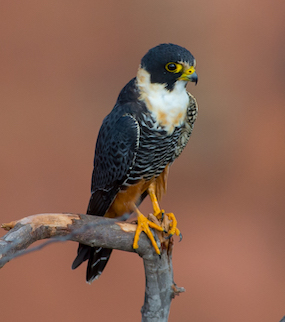
\includegraphics{./FALCO.jpeg}

\hypertarget{objetivo}{%
\subsection{Objetivo}\label{objetivo}}

El objetivo del presente artículo es revelar cuál es la distribución
actual y potencial a futuro de F. rufigularis en México en función de
las variables bioclimáticas empleando una metodología que podría servir
no sólo para aumentar nuestro entendimiento sobre los patrones
biogeográficos de ésta especie, sino la de todo el género Falco,
permitiendo conocer si la distribución de la especie se mantendrá
constante en el tiempo o si habrá algún cambio considerable, así como
detalles en los patrones de su distribución que sólo es posible conocer
gracias a 1) la existencia de datos colectados de forma colectiva y
sistemática durante largos periodos de tiempo y 2) el uso de técnicas
estadísticas y de aprendizaje de máquina (Machine Learning) que permiten
procesar estos datos y encontrar patrones donde de otra forma podrían
pasar desapercibidos (Kelling et al.~2013).

\hypertarget{metodologuxeda}{%
\subsection{Metodología}\label{metodologuxeda}}

\hypertarget{obtenciuxf3n-y-pre-procesamiento-de-datos}{%
\subsubsection{Obtención y pre-procesamiento de
datos}\label{obtenciuxf3n-y-pre-procesamiento-de-datos}}

Los datos empleados para el análisis se obtuvieron de la base de datos
de eBird (eBird Basic Dataset, 2021), obteniendo los registros de F.
rufigularis para los años 2010-2020 a lo largo de todo el país. El
procesamiento de datos en éste trabajo se realizó empleando los
lenguajes de programación R y Python. Una vez obtenida la base, se
empleó el paquete de R AUK para procesar los datos, eliminando registros
duplicados debido a las listas compartidas por observadores y
manteniendo únicamente registros correspondientes al periodo de años
2010-2020.

\hypertarget{visualizaciuxf3n-de-los-registros}{%
\paragraph{Visualización de los
registros}\label{visualizaciuxf3n-de-los-registros}}

\includegraphics{falco_rufigularis_files/figure-latex/unnamed-chunk-2-1.pdf}

Además, dado el sesgo en la distribución de registros de observaciones
en eBird (sesgo de muestreo) y con el fin de generar un modelo
estadísticamente más confiable, se realizó un filtrado espacial
empleando el paquete de R spThin, obteniendo con el algoritmo un punto
por cada cinco kilómetros, y disminuyendo así la autocorrelación
espacial en las observaciones, realizando finalmente los modelos con 669
registros.

\begin{Shaded}
\begin{Highlighting}[]
\NormalTok{thinned\_dataset\_full }\OtherTok{\textless{}{-}} \FunctionTok{thin}\NormalTok{( }\AttributeTok{loc.data =}\NormalTok{ halcones, }
        \AttributeTok{lat.col =} \StringTok{"latitude"}\NormalTok{, }\AttributeTok{long.col =} \StringTok{"longitude"}\NormalTok{, }
        \AttributeTok{spec.col =} \StringTok{"common\_name"}\NormalTok{, }\CommentTok{\#campo con la especie}
        \AttributeTok{thin.par =} \DecValTok{5}\NormalTok{, }\AttributeTok{reps =} \DecValTok{10}\NormalTok{, }\CommentTok{\#thin par es la distancia en km para separar los puntos}
        \AttributeTok{locs.thinned.list.return =} \ConstantTok{TRUE}\NormalTok{, }
        \AttributeTok{write.files =}\NormalTok{ F, }
        \AttributeTok{max.files =} \DecValTok{5}\NormalTok{, }\CommentTok{\#Numero de posibles soluciones de seleccion}
        \AttributeTok{out.dir =} \StringTok{"XXX"}\NormalTok{, }
        \AttributeTok{out.base =} \StringTok{"bat\_thinned"}\NormalTok{, }
        \AttributeTok{write.log.file =} \ConstantTok{TRUE}\NormalTok{,}
        \AttributeTok{log.file =} \StringTok{"bat\_thinned\_file.txt"}\NormalTok{ ) }\CommentTok{\#un resumen del proceso y sus resultados}


\NormalTok{ bat }\OtherTok{\textless{}{-}}\NormalTok{ thinned\_dataset\_full[}\DecValTok{1}\NormalTok{] }\SpecialCharTok{\%\textgreater{}\%} 
        \FunctionTok{as.data.frame}\NormalTok{()}
\end{Highlighting}
\end{Shaded}

\hypertarget{modelo-de-distribucion-espacial}{%
\subsubsection{Modelo de distribucion
espacial}\label{modelo-de-distribucion-espacial}}

Se realizó un modelo de nicho ecológico para la especie, considerando
las 19 variables ambientales de WorldClim, las cuales fueron: (BIO1)
temperatura media anual, (BIO2) rango diurno medio, (BIO3)
isotermalidad, (BIO4) estacionalidad de la temperatura, (BIO5)
temperatura máxima del mes más cálido, (BIO6) temperatura mínima del mes
más frío, (BIO7) rango anual de temperatura, (BIO8) temperatura media
del trimestre más húmedo, (BIO9) temperatura media del cuarto más seco,
(BIO10) temperatura media del trimestre más cálido, (BIO11) temperatura
media del cuarto más frío, (BIO12) precipitación anual, (BIO13)
precipitación del mes más húmedo, (BIO14) precipitación del mes más
seco, (BIO15) estacionalidad de la precipitación, (BIO16) precipitación
del cuarto más húmedo, (BIO17) precipitación del cuarto más seco,
(BIO18) precipitación del trimestre más cálido, (BIO19) precipitación
del cuarto más frío. Para implementar esto fue necesario el uso de las
librerias especializdas maptools, raster y dismo.

\begin{Shaded}
\begin{Highlighting}[]
\FunctionTok{library}\NormalTok{(rsample)}
\FunctionTok{library}\NormalTok{ (maptools)}
\FunctionTok{library}\NormalTok{(raster)}
\FunctionTok{library}\NormalTok{(dismo)}
\FunctionTok{library}\NormalTok{(randomForest)}
\FunctionTok{library}\NormalTok{(rpart)}
\FunctionTok{library}\NormalTok{(ggplot2)}

\FunctionTok{set.seed}\NormalTok{(}\DecValTok{0}\NormalTok{)}
\NormalTok{bat }\OtherTok{\textless{}{-}} \FunctionTok{read.csv}\NormalTok{(}\StringTok{"./bat\_thinned\_file.csv"}\NormalTok{, }\AttributeTok{header =} \ConstantTok{TRUE}\NormalTok{)}

\FunctionTok{data}\NormalTok{(}\StringTok{"wrld\_simpl"}\NormalTok{)}

\CommentTok{\# variables  bioclimaticas predictoras  }
\NormalTok{wc }\OtherTok{\textless{}{-}}\NormalTok{ raster}\SpecialCharTok{::}\FunctionTok{getData}\NormalTok{(}\StringTok{"worldclim"}\NormalTok{, }\AttributeTok{var =} \StringTok{"bio"}\NormalTok{, }\AttributeTok{res =} \DecValTok{10}\NormalTok{)}

\CommentTok{\# extraer datos climáticos de las ubicaciones de nuestras observaciones. }
\NormalTok{clima\_bat }\OtherTok{\textless{}{-}}\NormalTok{ raster}\SpecialCharTok{::}\FunctionTok{extract}\NormalTok{(wc, bat[,}\DecValTok{1}\SpecialCharTok{:}\DecValTok{2}\NormalTok{]) }
\FunctionTok{head}\NormalTok{(clima\_bat)}
\end{Highlighting}
\end{Shaded}

\begin{verbatim}
##      bio1 bio2 bio3 bio4 bio5 bio6 bio7 bio8 bio9 bio10 bio11 bio12 bio13 bio14
## [1,]  253  118   62 2194  344  155  189  263  251   276   221  1174   227    26
## [2,]  248  118   62 2248  339  149  190  259  245   271   215  1118   199    24
## [3,]  250  107   60 2091  334  158  176  260  247   271   219  1226   215    30
## [4,]  246  110   61 2163  333  153  180  257  243   268   215  1202   206    30
## [5,]  252  109   61 2086  338  160  178  262  250   275   222  1244   233    30
## [6,]  248  118   62 2248  339  149  190  259  245   271   215  1118   199    24
##      bio15 bio16 bio17 bio18 bio19
## [1,]    63   535    88   294   126
## [2,]    59   468    93   308   129
## [3,]    57   516   100   323   147
## [4,]    56   493   101   325   146
## [5,]    60   554    98   315   143
## [6,]    59   468    93   308   129
\end{verbatim}

\begin{Shaded}
\begin{Highlighting}[]
\CommentTok{\# añado columna de presencia 1 / ausencia 0 }
\NormalTok{pa }\OtherTok{\textless{}{-}} \FunctionTok{c}\NormalTok{(}\FunctionTok{rep}\NormalTok{(}\DecValTok{1}\NormalTok{, }\DecValTok{668}\NormalTok{)) }
\NormalTok{clima\_bat }\OtherTok{\textless{}{-}} \FunctionTok{cbind}\NormalTok{(clima\_bat, pa)}

\DocumentationTok{\#\#\#\# análisis exploratorio }
\FunctionTok{plot}\NormalTok{(bat[,}\DecValTok{1}\SpecialCharTok{:}\DecValTok{2}\NormalTok{], }\AttributeTok{cex =} \FloatTok{0.5}\NormalTok{, }\AttributeTok{col =} \StringTok{"blue"}\NormalTok{)}
\FunctionTok{plot}\NormalTok{(wrld\_simpl, }\AttributeTok{add =}\NormalTok{ T)}
\end{Highlighting}
\end{Shaded}

\includegraphics{falco_rufigularis_files/figure-latex/unnamed-chunk-4-1.pdf}

\begin{Shaded}
\begin{Highlighting}[]
\CommentTok{\# BIo 1: Annual Mean Temperature }
\CommentTok{\# Bio 12: Annual precipitation }
\FunctionTok{plot}\NormalTok{(clima\_bat[,}\DecValTok{1}\NormalTok{]}\SpecialCharTok{/}\DecValTok{10}\NormalTok{, clima\_bat[,}\DecValTok{12}\NormalTok{], }\AttributeTok{xlab =} \StringTok{"Bio1"}\NormalTok{, }\AttributeTok{ylab =} \StringTok{"Bio12"}\NormalTok{)}
\end{Highlighting}
\end{Shaded}

\includegraphics{falco_rufigularis_files/figure-latex/unnamed-chunk-4-2.pdf}

\begin{Shaded}
\begin{Highlighting}[]
\DocumentationTok{\#\#\# modelamiento de presencia vs random expectation. }
\CommentTok{\# definicion random expectation: también llamada background, o random absence data, }
\CommentTok{\# es lo que obtendrías si la especie no tuviera ninguna preferencia por ninguna de }
\CommentTok{\# las variables predictora (u otras variables que no estén correlacionadas con las }
\CommentTok{\# variables predictoras).}

\CommentTok{\# la extensión de la distribución de la especie}
\NormalTok{ext }\OtherTok{\textless{}{-}}\NormalTok{ raster}\SpecialCharTok{::}\FunctionTok{extent}\NormalTok{(}\FunctionTok{SpatialPoints}\NormalTok{(bat[,}\DecValTok{1}\SpecialCharTok{:}\DecValTok{2}\NormalTok{]))}

\NormalTok{mex }\OtherTok{\textless{}{-}} \FunctionTok{getData}\NormalTok{(}\StringTok{"GADM"}\NormalTok{, }\AttributeTok{country =} \StringTok{"MEX"}\NormalTok{, }\AttributeTok{level =} \DecValTok{1}\NormalTok{)}

\CommentTok{\# generamos 3000 muestras aleatorias de extent }
\NormalTok{random\_ar }\OtherTok{\textless{}{-}} \FunctionTok{sampleRandom}\NormalTok{(wc, }\DecValTok{3000}\NormalTok{, }\AttributeTok{ext =}\NormalTok{ ext) }\CommentTok{\# ext = para limitar el muestreo al}
\CommentTok{\# área dentro de la extensión. }

\CommentTok{\# generamos columna de presencia 1 ausencia 0 }
\NormalTok{par }\OtherTok{\textless{}{-}} \FunctionTok{c}\NormalTok{(}\FunctionTok{rep}\NormalTok{(}\DecValTok{0}\NormalTok{, }\DecValTok{3000}\NormalTok{))}
\NormalTok{random\_ar }\OtherTok{\textless{}{-}} \FunctionTok{cbind}\NormalTok{(random\_ar, par)}

\NormalTok{bat\_completor }\OtherTok{\textless{}{-}} \FunctionTok{rbind}\NormalTok{(clima\_bat, random\_ar) }\SpecialCharTok{\%\textgreater{}\%} 
  \FunctionTok{as.data.frame}\NormalTok{() }

\NormalTok{bat\_split }\OtherTok{\textless{}{-}} \FunctionTok{initial\_split}\NormalTok{(bat\_completor, }\AttributeTok{strata =}\NormalTok{ pa)}
\NormalTok{train\_data }\OtherTok{\textless{}{-}} \FunctionTok{training}\NormalTok{(bat\_split)}
\NormalTok{test\_data }\OtherTok{\textless{}{-}} \FunctionTok{testing}\NormalTok{(bat\_split)}

\NormalTok{cart }\OtherTok{\textless{}{-}} \FunctionTok{rpart}\NormalTok{(pa}\SpecialCharTok{\textasciitilde{}}\NormalTok{., }\AttributeTok{data=}\NormalTok{train\_data)}

\CommentTok{\#para encontrar el hiperparametro mtry}
\NormalTok{trf }\OtherTok{\textless{}{-}} \FunctionTok{tuneRF}\NormalTok{(train\_data[, }\DecValTok{1}\SpecialCharTok{:}\DecValTok{19}\NormalTok{], train\_data[, }\StringTok{\textquotesingle{}pa\textquotesingle{}}\NormalTok{])}
\end{Highlighting}
\end{Shaded}

\begin{verbatim}
## mtry = 6  OOB error = 0.1237212 
## Searching left ...
## mtry = 3     OOB error = 0.1209218 
## 0.02262607 0.05 
## Searching right ...
## mtry = 12    OOB error = 0.1221528 
## 0.01267647 0.05
\end{verbatim}

\includegraphics{falco_rufigularis_files/figure-latex/unnamed-chunk-4-3.pdf}

\begin{Shaded}
\begin{Highlighting}[]
\NormalTok{mt }\OtherTok{\textless{}{-}}\NormalTok{ trf[}\FunctionTok{which.min}\NormalTok{(trf[,}\DecValTok{2}\NormalTok{]), }\DecValTok{1}\NormalTok{]}
\NormalTok{mt}
\end{Highlighting}
\end{Shaded}

\begin{verbatim}
## [1] 3
\end{verbatim}

\begin{Shaded}
\begin{Highlighting}[]
\NormalTok{rrf }\OtherTok{\textless{}{-}} \FunctionTok{randomForest}\NormalTok{(train\_data[, }\DecValTok{1}\SpecialCharTok{:}\DecValTok{19}\NormalTok{], train\_data[, }\StringTok{\textquotesingle{}pa\textquotesingle{}}\NormalTok{], }\AttributeTok{mtry=}\NormalTok{mt)}
\FunctionTok{plot}\NormalTok{(rrf)}
\end{Highlighting}
\end{Shaded}

\includegraphics{falco_rufigularis_files/figure-latex/unnamed-chunk-4-4.pdf}

\begin{Shaded}
\begin{Highlighting}[]
\FunctionTok{varImpPlot}\NormalTok{(rrf)}
\end{Highlighting}
\end{Shaded}

\includegraphics{falco_rufigularis_files/figure-latex/unnamed-chunk-4-5.pdf}

\begin{Shaded}
\begin{Highlighting}[]
\NormalTok{eva }\OtherTok{\textless{}{-}} \FunctionTok{evaluate}\NormalTok{(test\_data[test\_data}\SpecialCharTok{$}\NormalTok{pa}\SpecialCharTok{==}\DecValTok{1}\NormalTok{, ], test\_data[test\_data}\SpecialCharTok{$}\NormalTok{pa}\SpecialCharTok{==}\DecValTok{0}\NormalTok{, ], rrf)}
\NormalTok{eva}
\end{Highlighting}
\end{Shaded}

\begin{verbatim}
## class          : ModelEvaluation 
## n presences    : 167 
## n absences     : 750 
## AUC            : 0.8258802 
## cor            : 0.4434351 
## max TPR+TNR at : 0.1391333
\end{verbatim}

\begin{Shaded}
\begin{Highlighting}[]
\FunctionTok{plot}\NormalTok{(eva, }\StringTok{\textquotesingle{}ROC\textquotesingle{}}\NormalTok{)}
\end{Highlighting}
\end{Shaded}

\includegraphics{falco_rufigularis_files/figure-latex/unnamed-chunk-4-6.pdf}

\begin{Shaded}
\begin{Highlighting}[]
\CommentTok{\#predictions}
\NormalTok{rp }\OtherTok{\textless{}{-}} \FunctionTok{predict}\NormalTok{(wc, rrf, }\AttributeTok{ext=}\NormalTok{mex)}
\FunctionTok{plot}\NormalTok{(rp)}
\end{Highlighting}
\end{Shaded}

\includegraphics{falco_rufigularis_files/figure-latex/unnamed-chunk-4-7.pdf}

\hypertarget{regionalizaciuxf3n-de-poblaciones}{%
\subsubsection{Regionalización de
poblaciones}\label{regionalizaciuxf3n-de-poblaciones}}

Para entender la distribución de la especie en el país y su potencial
agrupamiento en subpoblaciones, se aplicó un algoritmo DBSCAN
(Density-Based Spatial Clustering of Applications with Noise, por sus
siglas en inglés), una técnica de agrupamiento de aprendizaje de máquina
basado en densidad de puntos que permite clasificar en grupos datos no
etiquetados de forma no supervisada y que tiene un desempeño apropiado
con datos espaciales . DBSCAN requiere de tres parámetros (en el
contexto del Machine Learning, hiper parámetros) que fueron definidos
por nosotros; 1) un valor epsilon, que es el criterio de distancia
mínima entre dos puntos para ser considerados vecinos y formar un grupo
(subpoblación en el contexto del presente trabajo), 2) mínimo de
muestras, que es la cantidad mínima de registros agrupados para ser
considerados un grupo y no valores atípicos (registros aislados) y 3)
una métrica para calcular la distancia entre puntos.

\begin{figure}
\centering
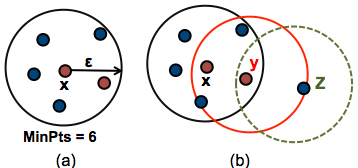
\includegraphics{./dbscan-principle.png}
\caption{Visualización de algoritmo DBSCAN.}
\end{figure}

Para elegir el valor más apropiado para epsilon, se realizó primero un
modelo de vecinos más cercanos (Nearest Neighbours), otro algoritmo de
aprendizaje de máquina que agrupa los datos en función de un número de
clusters determinado por el investigador, permitiendo calcular la
distancia a los n puntos más cercanos de cada registro, ordenarlos y
posteriormente graficarlos para observar el valor óptimo de epsilon, el
cual se ve reflejado como el punto de máxima curvatura.

\begin{Shaded}
\begin{Highlighting}[]
\ImportTok{import}\NormalTok{ pandas }\ImportTok{as}\NormalTok{ pd}
\ImportTok{import}\NormalTok{ numpy }\ImportTok{as}\NormalTok{ np}
\ImportTok{import}\NormalTok{ matplotlib.pyplot }\ImportTok{as}\NormalTok{ plt}
\ImportTok{import}\NormalTok{ seaborn }\ImportTok{as}\NormalTok{ sns}
\ImportTok{from}\NormalTok{ sklearn.neighbors }\ImportTok{import}\NormalTok{ NearestNeighbors}
\ImportTok{from}\NormalTok{ sklearn.cluster }\ImportTok{import}\NormalTok{ DBSCAN}
\ImportTok{import}\NormalTok{ geopandas }\ImportTok{as}\NormalTok{ gpd}

\CommentTok{\# aquí hay que conectar la tubería, en el chunk anterior se crea el objeto bat como data frame en R. Aquí hay que conectar ese data frame con un pandas data frame.}

\NormalTok{bat }\OperatorTok{=}\NormalTok{ pd.read\_csv(}\StringTok{"./Bat\_thinned\_file.csv"}\NormalTok{)}

\CommentTok{\# la primera columna del arreglo debe ser latitud}
\NormalTok{latitud }\OperatorTok{=}\NormalTok{ bat[}\StringTok{"latitude"}\NormalTok{]}

\CommentTok{\# la segunda columna del arreglo debe ser longitud}
\NormalTok{longitud }\OperatorTok{=}\NormalTok{ bat[}\StringTok{"longitude"}\NormalTok{]}

\CommentTok{\# creo un data frame con el orden necesario:}
\NormalTok{bat }\OperatorTok{=}\NormalTok{ pd.DataFrame([latitud, longitud]).transpose()}

\CommentTok{\# Ajustamos el modelo de Nearest Neighbours transformando los valores en radianes}
\NormalTok{neigh }\OperatorTok{=}\NormalTok{ NearestNeighbors(metric }\OperatorTok{=} \StringTok{\textquotesingle{}haversine\textquotesingle{}}\NormalTok{, n\_neighbors}\OperatorTok{=}\DecValTok{5}\NormalTok{)}
\NormalTok{nbrs }\OperatorTok{=}\NormalTok{ neigh.fit(np.radians(bat))}
\NormalTok{distances, \_ }\OperatorTok{=}\NormalTok{ nbrs.kneighbors(np.radians(bat))}

\CommentTok{\# Ordenamos las distancias de menor a mayor y observamos el punto (distancia) donde se presenta la mayor curvatura (punto de inflexión en las distancias)}
\NormalTok{distances }\OperatorTok{=}\NormalTok{ np.sort(distances, axis}\OperatorTok{=}\DecValTok{0}\NormalTok{)}
\NormalTok{distances }\OperatorTok{=}\NormalTok{ distances[:,}\DecValTok{1}\NormalTok{]}
\NormalTok{plt.plot(distances)}
\NormalTok{plt.xlabel(}\StringTok{"Distancia"}\NormalTok{)}
\NormalTok{plt.ylabel(}\StringTok{"Epsilon"}\NormalTok{)}
\NormalTok{plt.title(}\StringTok{"K distancias"}\NormalTok{, fontsize}\OperatorTok{=}\DecValTok{20}\NormalTok{)}
\NormalTok{plt.show()}
\end{Highlighting}
\end{Shaded}

\begin{figure}
\centering
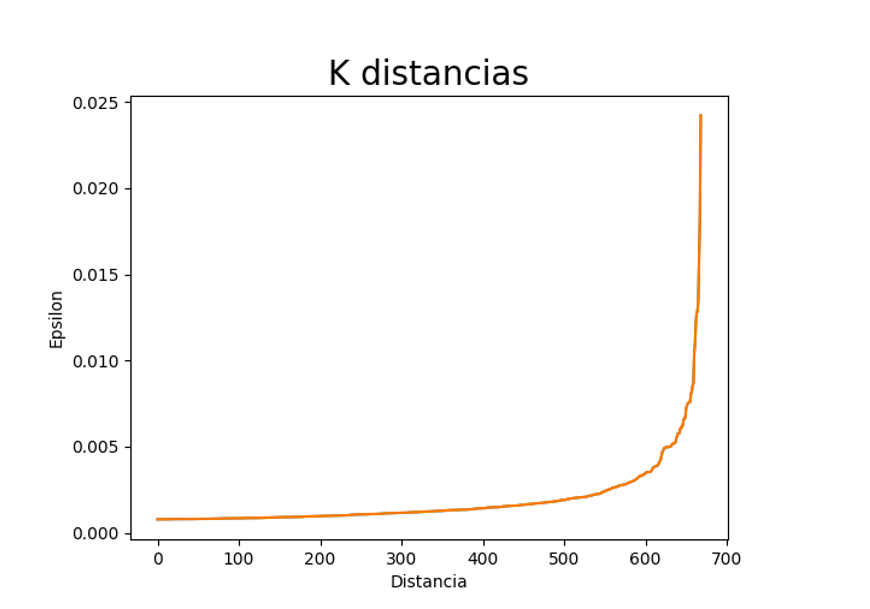
\includegraphics{./KMEANS.png}
\caption{Curva de puntos ordenados por distancia para determinación del
parámetro épsilon.}
\end{figure}

\begin{Shaded}
\begin{Highlighting}[]
\CommentTok{\# Ajustamos el modelo transformando los valores en radianes}
\NormalTok{dbscan }\OperatorTok{=}\NormalTok{ DBSCAN(eps}\OperatorTok{=}\FloatTok{0.010}\NormalTok{, min\_samples}\OperatorTok{=}\DecValTok{4}\NormalTok{, metric}\OperatorTok{=}\StringTok{\textquotesingle{}haversine\textquotesingle{}}\NormalTok{) }\CommentTok{\# mejores parámetros so far: eps=0.010, min=4}

\CommentTok{\# vale la pena explorar más combinaciones...}
\NormalTok{dbscan.fit(np.radians(bat))}

\CommentTok{\# Obtenemos la etiqueta del clúster para cada observación}
\NormalTok{clusters }\OperatorTok{=}\NormalTok{ dbscan.labels\_}

\CommentTok{\#\# parte espacial: mapa de mexico (CARGAR .SHAPE DE MÉXICO). }
\NormalTok{mexico }\OperatorTok{=}\NormalTok{ gpd.read\_file(}\StringTok{".shp"}\NormalTok{)}

\CommentTok{\#\# grafica sobre mapa}
\NormalTok{ax }\OperatorTok{=}\NormalTok{ mexico.plot(color }\OperatorTok{=} \StringTok{"lightgrey"}\NormalTok{, linestyle }\OperatorTok{=} \StringTok{":"}\NormalTok{, edgecolor }\OperatorTok{=} \StringTok{"black"}\NormalTok{)}
\NormalTok{sns.scatterplot(data }\OperatorTok{=}\NormalTok{ bat, x }\OperatorTok{=}\StringTok{"longitude"}\NormalTok{, y }\OperatorTok{=} \StringTok{"latitude"}\NormalTok{, hue }\OperatorTok{=}\NormalTok{ clusters,  palette}\OperatorTok{=}\StringTok{"rainbow"}\NormalTok{, ax}\OperatorTok{=}\NormalTok{ax)}
\NormalTok{plt.xlabel(}\StringTok{"Longitud"}\NormalTok{)}
\NormalTok{plt.ylabel(}\StringTok{"Latitud"}\NormalTok{)}
\NormalTok{plt.title(}\StringTok{"Grupos obtenidos con DBSCAN"}\NormalTok{, fontsize}\OperatorTok{=}\DecValTok{20}\NormalTok{)}
\NormalTok{plt.show()}
\end{Highlighting}
\end{Shaded}

\begin{figure}
\centering
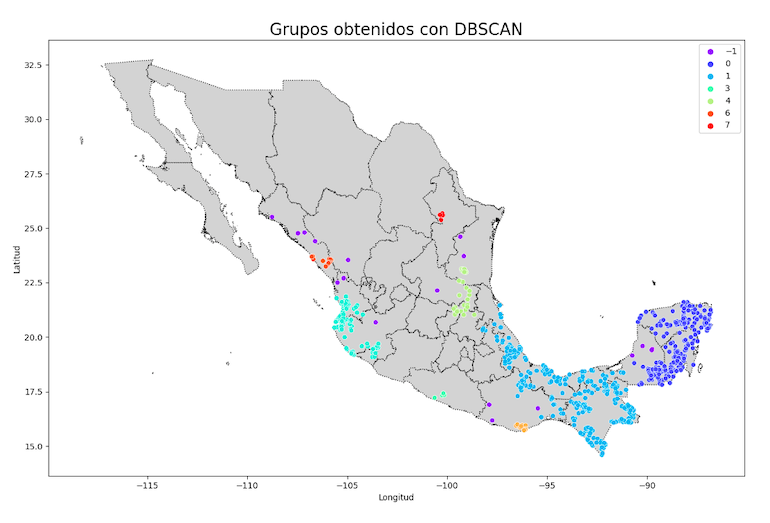
\includegraphics{./MAP.png}
\caption{Agrupamiento de registros de F. rufigularis con el algoritmo
DBSCAN.}
\end{figure}

\hypertarget{resultados}{%
\subsection{Resultados}\label{resultados}}

Falco rufigularis es una especie que se encuentra principalmente en la
parte sur del país, mostrando una continua idoneidad en las costas y en
la península de Yucatán (el modelo generado tiene un AUC de 0.90 ).

Respecto al agrupamiento de los registros, el algoritmo DBSCAN arrojó
ocho grupos, con lo cual podríamos entender que la población total de F.
rufigularis en México se divide en 8 subpoblaciones (etiquetadas de cero
a siete). En color morado y con etiqueta -1, se representan los datos
atípicos (o ruido, en el contexto de éste algoritmo), los cuales son
registros que no cumplieron con el criterio de permanencia a ningún
grupo por la proximidad.

\hypertarget{conclusiuxf3n}{%
\subsection{Conclusión}\label{conclusiuxf3n}}

El halcón murcielaguero presenta una amplia distribución en México, la
cual está altamente correlacionada con la idoneidad ambiental para la
especie. Sus poblaciones más abundantes y extensas se encuentran en el
sureste del país, la cual es una región con fuertes presiones
antropogénicas. Debido a su abundancia y distribución en la región
neotropical en el país, así como a su sensibilidad a la perturbación, es
posible que ésta especie sea un buen indicador ambiental para conocer el
impacto de las actividades antropogénicas en otras rapaces tropicales
presentes en la región pero que debido a menor densidad poblacional y
hábitos más esquivos son difíciles de estudiar y monitorear. Por otro
lado, los modelos de agrupamiento no supervisado resultaron ser una gran
herramienta para analizar los patrones espaciales en la distribución de
la especie, por lo que se sugiere su uso al momento de analizar datos de
otras especies.

\end{document}
